\documentclass[10pt,onecolumn,journal,draftclsnofoot]{IEEEtran}
\usepackage[margin=0.75in]{geometry}
\usepackage{listings}
\usepackage{color}
\usepackage{longtable}
\usepackage{graphicx}
\usepackage{float}
\usepackage{tabu}
\usepackage{enumitem}
\usepackage{courier}
\usepackage{hyperref}
\usepackage{parskip}
\definecolor{dkgreen}{rgb}{0,0.6,0}
\definecolor{gray}{rgb}{0.5,0.5,0.5}
\definecolor{mauve}{rgb}{0.58,0,0.82}

\graphicspath{{../images/}}

%Subsection headers to Arabic numerals
%\renewcommand\thesection{\arabic{section}}
%\renewcommand\thesubsection{\thesection.\arabic{subsection}}
%\renewcommand\thesubsubsection{\thesubsection.\arabic{subsubsection}}

%Section headers to Arabic numerals
%\renewcommand\thesectiondis{\arabic{section}}
%\renewcommand\thesubsectiondis{\thesectiondis.\arabic{subsection}}
%\renewcommand\thesubsubsectiondis{\thesubsectiondis.\arabic{subsubsection}}

%Remove numbering from the bibliography section

\lstset{frame=none,
language=C,
columns=flexible,
numberstyle=\tiny\color{gray},
keywordstyle=\color{blue},
commentstyle=\color{dkgreen},
stringstyle=\color{mauve},
breaklines=true,
breakatwhitespace=true,
tabsize=4,
showstringspaces=false,
basicstyle=\ttfamily
}

\setlength{\parindent}{0cm}

\begin{document}

\begin{titlepage}
	\title{Intel Cloud Orchestration Networking\\ Winter Midterm Progress Report}
	\author{Matthew~Johnson,~Cody~Malick,~and~Garrett~Smith\\
		Team 51, Cloud Orchestra}
	\date{\today}
	\markboth{Senior Design, CS 461, Winter 2017}{}
	\maketitle
	\vspace{4cm}
	\begin{abstract}
		\noindent This document outlines the progress of the Cloud
		Orchestration Networking project over the Fall and Winter
		terms. It contains a short description of the project's purposes
		and goals, current progress, current issues, and any solutions
		to those issues. It also contains a week by week retrospective
		for all ten weeks of Fall term and the first half of Winter
		term. \end{abstract}

\end{titlepage}
\tableofcontents
\clearpage

\section{Project Goals}

Our project is to first switch the Linux-created GRE tunnel implementation in
Ciao to use GRE tunnels created by Open vSwitch. From that point we will switch
the actual tunneling implementation from GRE to VxLAN/nvGRE based on performance
measurements of each on data center networking cards. After this is completed, a
stretch goal is to replace Linux bridges with Open vSwitch switch instances.

\section{Purpose}

The current implementation of Ciao tightly integrates software defined
networking principles to leverage a limited local awareness of just enough of
the global cloud's state. Tenant overlay networks are used to overcome
traditional hardware networking challenges by using a distributed, stateless,
self-configuring network topology running over dedicated network software
appliances. This design is achieved using Linux-native Global Routing
Encapsulation (GRE) tunnels and Linux bridges, and scales well in an environment
of a few hundred nodes.

While this initial network implementation in Ciao satisfies current simple
networking needs in Ciao, all innovation around software defined networks has
shifted to the Open vSwitch (OVS) framework. Moving Ciao to OVS will allow
leverage of packet acceleration frameworks like the Data Plane Development Kit
(DPDK) as well as provide support for multiple tunneling protocols such as VxLAN
and nvGRE. VxLAN and nvGRE are equal cost multipath routing (ECMP) friendly,
which could increase network performance overall.

\section{Fall Progress}
At present, the project is moving along smoothly. Our testing environment has
been set up and is networked appropriately. Each Intel NUC (Next Unit of
Computing) has Clear Linux installed. Come Winter term, we will get Ciao set up
on each machine and begin development on Ciao. Software development on the
project has yet to begin as we have just wrapped up the design phase.

Designing has been quite helpful in developing our understanding of the project,
its goals, and purpose. Because this is a small component of a very complicated
system, taking the time to investigate what a software defined network is, why
it's being used, and why we are implementing the piece that we are has been
quite beneficial.

While in the design phase, we found an extremely useful library for interfacing
with Open vSwitch, libovsdb. Libovsdb is a library written in the Go programming
language that allows for simple and efficient calls to the OVS Database
Management Protocol. Interfacing with OVS is going to be a very large
portion of the project for us, so finding the library is quite the boon. Here
is a quick example of how this library functions:\cite{gosample}\\

\begin{lstlisting}[caption=Example insert operation using libovsdb]
	// simple insert operation
	insertOp := libovsdb.Operation{
		Op:	  "insert",
		Table:	  "Bridge",
		Row:	  bridge,
		UUIDName: namedUUID,
	}
\end{lstlisting}

The above example can be reused for all major operations in the OVS Database
Management Protocol. Other example operations include select, delete, and
update. Using just the operations listed here, we can accomplish most of the
needed configuration changes within Open vSwitch.

\section{Fall Term Week by Week Reports}
%just paste in weekly blogs?

\subsection{Background}

Over the Summer, 2016, Matthew worked as a Software Engineering Intern for the
Advanced Systems Engineering (ASE) group within the Open Source Technology
Center (OTC) that is in turn within the Software Services Group (SSG) at Intel.
Matthew's coworkers had a need to integrate Open vSwitch in their cloud
orchestration software (Cloud Integrated Advanced Orchestrator, or Ciao) but did
not have the man hours to contribute time to it. Matthew worked with the team to
propose the project as a Senior Capstone project at Oregon State University.

Matthew identified two other students, Cody Malick and Garrett Smith, as
intelligent hard workers who would benefit the project. Because of this Robert
Nesius, the Intel Engineering Manager serving as our client, requested Matthew,
Cody, and Garrett specifically for this project.

\subsection{Weeks Zero Through Two}

During the first week of class, we all visited Intel in Hillsboro. The principal
engineer in charge of Ciao networking, Manohar Castelino, gave us all an
explanation of Ciao, how the networking works, and what he expects us to
accomplish.

It was also during this time that Rob provided us with five Intel NUCs that
would serve as our local cluster. We found out that we needed to register the
MAC addresses with the university, and communicated this need to Todd Shechter,
the Oregon State University Director of Information Technology.

\subsection{Week Three}

During week three we attempted to install Clear Linux OS for Intel
Architecture~\cite{clearlinux} on all five Intel NUCs. We were unsuccessful
because the installer requires a network connection to download the packaging.
At this point, network access had yet to be approved by OSU IT.

Network access is required to install Clear Linux, Ciao, and access the machines
remotely. Since Clear Linux is a datacenter OS, not a desktop OS, it does not
support wireless internet connections. Because ethernet is required our hardware
must be registered with the university. If we were unable to obtain network
access for the hardware on OSU's network we would have needed to find somewhere
else to house it.

We also wrote our problem statement in week three, earlier than most groups were
able to, since we were ahead of schedule with regard to meeting our team and
choosing a project.

\subsection{Week Four}

During week four Matthew installed Clear Linux on the Intel NUCs. Since there
the networking issues had still not been solved he brought them to his house to
use the wired connection there. At this point our hardware had been registered
with the university, but for unknown reasons our NUCs were not connecting to the
network. Todd Shechter was devoting a lot of his time to help us debug, but we
were not yet successful. He set us up with two five-port switches in Kevin
McGrath's lab, but they were not receiving IP addresses from the network.

We had our problem statement reviewed and were waiting for feedback by the end
of the week. We also started working on the client requirements document, though
much of our contributions were simple outline and templating work.

\subsection{Week Five}

This week we spent most of our time writing the rough draft for the requirements
document. We turned it in by the end of the week and were satisfied with our
progress. The final draft of the requirements document was due the next week,
week six. This week we also turned in our signed copy of the problem statement.

This week our networking issues were resolved. We had another email conversation
with Todd Shechter, who was at a loss as to why we could not access the network
from the NUCs. He granted us access to an HP switch we had successfully
connected via in the past. On Thursday, we went to move all our NUCs to the new
switch, but tried out the network on the mini switches one last time. This time
they all worked. Our hardware was now set up and ready to go.

\subsection{Week Six}

This week we finished writing the requirements document that was due at the end
of the week. After the rough draft we turned in the previous week we continued
working on it ourselves until Tuesday. On Wednesday Frank emailed us some
suggestions and we addressed those right away. We got the document signed that
afternoon by Rob Nesius, our client at Intel.

\subsection{Week Seven}

This week we started working on the technical review document due the following
Monday. This document outlines nine different components of our system. For each
component we explored three different technologies that could be used to
implement the component. Since our project is implementing a component of a
larger system, it was difficult for us to come up with nine components and three
technologies each (twenty-seven different options). We spent much of our week
working together to figure out how to split the project up.

\subsection{Week Eight}

This week we submitted the tech review document. It was a lot of work, but we
got it in on time unlike many other capstone groups. Garrett researched software
switch options, network latency tools, and network throughput tools. Matthew
dealt with high-level language, testing, and logging tools. Cody handled the
network-specific implementation pieces, such as packet protocols, network
virtualization implementation, and bridge implementation.

\subsection{Week Nine}

This was a short week with Thursday and Friday given over to the Thanksgiving
holiday. We started working on the design document but did not make much headway
before breaking for the holiday weekend.

Our team also got together and talked about how we were going to execute the
final presentation video for a few minutes this week.

\subsection{Week Ten}

This week we focused on the design document due Friday. We spent time
researching design strategies and writing up our plan to execute. During this
research we found a very useful Go library that interfaces with Open vSwitch.
This library will simplify our implementation, allowing us more time to do
network performance testing, which the client is very interested in. Our client
signed the document with a half-hour to spare before the deadline, and the
technical advisors for the project, Manohar Castelino and Tim Pepper, indicated
they were impressed with the design we had outlined.

\section{Fall Term Retrospective}

\begin{center}
	\begin{tabular}{| p{0.05\linewidth} | p{0.3\linewidth} | p{0.3\linewidth} |
			p{0.3\linewidth} |}\hline
		Week & Positives & Deltas & Actions \\ \hline

		0-2 & Met the Intel team, studied project goals, purposes  &
			Write project abstract & Research project, write project
			abstract \\ \hline

		3 & Started testing hardware setup, problem statement
			first draft submitted & Resolve networking issues & 
			Contact Todd to get NUC network authorization, write
			final draft of problem statement\\ \hline

		4 & Completed hardware setup  & Get problem statement signed  &
			Email project owners and get problem statement approved
			\\ \hline

		5 & Problem statement submitted, completed first draft
			of requirements document & Submit final draft of
			requirements document & Update requirements document,
			email project owners, get approval via signature \\ 
			\hline

		6 & Final draft of requirements document submitted & Begin work
			on tech review & Research technologies for tech review 
			\\ \hline

		7 & First draft of tech review completed & Finalize tech review
			& Update and submit tech review \\ \hline

		8 & Submitted tech review & Begin design document & Research 
			project design steps and implementation details\\ \hline
		
		9 & Began work on design document & Complete design document  &
			Fill out the rest of the design document over 
			Thanksgiving weekend \\ \hline

		10 & Completed design document, began work on final report and
			final presentation & Complete final report, complete
			final presentation & Over the weekend, complete final
			report, create slides for final presentation\\ \hline

	\end{tabular}
\end{center}
\section{Winter Progress - Cody Malick}
Winter term has started off a little bumpy for the team. We spent the first 
four weeks focusing on setting up our development environment, as well as ironing
out issues related to network testing. These topics will be covered in-depth
in the folling 'issues' section. Our current progress, as far as development
is concerned, is working on the first feature, implementing OVS generated GRE
tunnels. While we originally planned to have that feature completed by the end
of the fifth week, we are in contact with our friends at Intel to figure out
some of the issues we've been running into. Good progress on testing the basic
NUC setup, and will be covered in the following section. Lastly, our current
development progress, and issues related to deployment of OVS in Ciao will
be discussed. 

\subsection{Network Testing Progress - Garrett Smith}
To help handle the data from the network testing tools iperf and qperf Garrett 
wrote some scripts in Ruby to convert the output from multiple runs of iperf 
and qperf into CSV files. Ruby was chosen because it has good support for 
consuming plain text and JSON (author's opinion), and because Garrett is 
familiar with it. The plain text support is useful because qperf outputs its 
results in human readable format which is not useful when comparing the results 
of multiple tests.
The JSON support is useful because we are using the iperf option to output 
results in JSON format, and again, we want to change the format the network 
performance data is in because the format is not great for using in performance 
comparisons.

We ran into more issues running the Ciao cluster on OSU's network so we 
moved it off of the OSU network. More details on those issues are in the Issues 
section. Garrett set up the Cisco SG300 switch Intel is 
lending us for this project in layer 3 mode and started up its built in DHCP 
server so we can run out own local area network that we have full control over.
This setup will be useful at expo because we will not have access to OSU's 
network while we are there.
The downsides this this setup 
are that we do not have remote access to the Nucs, and they cannot connect to 
the internet for updates.

Currently all of the Nucs have static IP addresses on the local network Garrett 
set up. We have not finished setting Ciao up on the new network yet. We need to 
clear out the configuration we had set for running Ciao on the OSU network 
before it will work correctly in the new configuration. We are in the process 
of setting up Ciao on the new network, but it has taken a lower priority than 
development.

\subsection{Development Progress - Matthew Johnson}

\section{Issues - Cody Malick}
In this section, we will cover the issues we ran into at the beginning of term,
as well as the solutions, and discussions that were had around them. The first
two major issues are related to environment setup. These two issues consumed a
large portion of the first part of the term.

\subsection{Environment Setup - Cody Malick}
The first, and arguably most major issue that was experienced, was setting up
the Ciao cluster. The first step of the project is, quite simply, getting Ciao
working in the state that it was provided to us. This ultimately should have
been fairly straightforward, but we ran into two major issues. The first of which
was the management of certificates in Clear Linux. 

Clear Linux, Intel's custom Linux distribution, is a fast OS designed to take
advantage of Intel CPU's advanced features that often go unutilized. This was
an obvious choice for our team. We initially set up all the NUCs with Clear Linux
installed, and proceeded with deployment. We spent about a week tracking down
an issue with Clear Linux. Specifically, that Clear Linux manually manages the
network trust store. This isn't an issue, but the behavior of Clear Linux was
slightly different than Ubuntu's. After some investigation, we reported the bug
to the Clear Linux team, who had a bug fix shipped in the next release.

The second major issue we encountered was that of getting FQDN's in Ciao, or
Fully Qualified Domain Names. These were important to the controller node of
Ciao as it needed to identify the compute nodes needed to deploy software onto.
As we were trying to deploy, we found that Ciao kept attempting to connect to
the hostname of the device instead of the FQDN. For example, the control node
would try to connect to \texttt{fw-dear205-ciao-nuc0} instead of the FQDN,
\texttt{fw-dear205-ciao-nuc0.engr.oregonstate.edu}. A screenshot of what is
expected of the python call is show below. At first, we thought this
issue was because of caching in the OS, but quickly found out this was not
the case after manually clearing the cache, as well as rebooting the system.
After some further investigation, we found that Python3 was only getting the
hostname on Clear Linux instead of the FQDN. We reported this problem to the
Clear Linux team as well, and they have since shipped a fix.

\begin{figure}[h]
	\caption{Expected result of Python FQDN call}
	\centering
	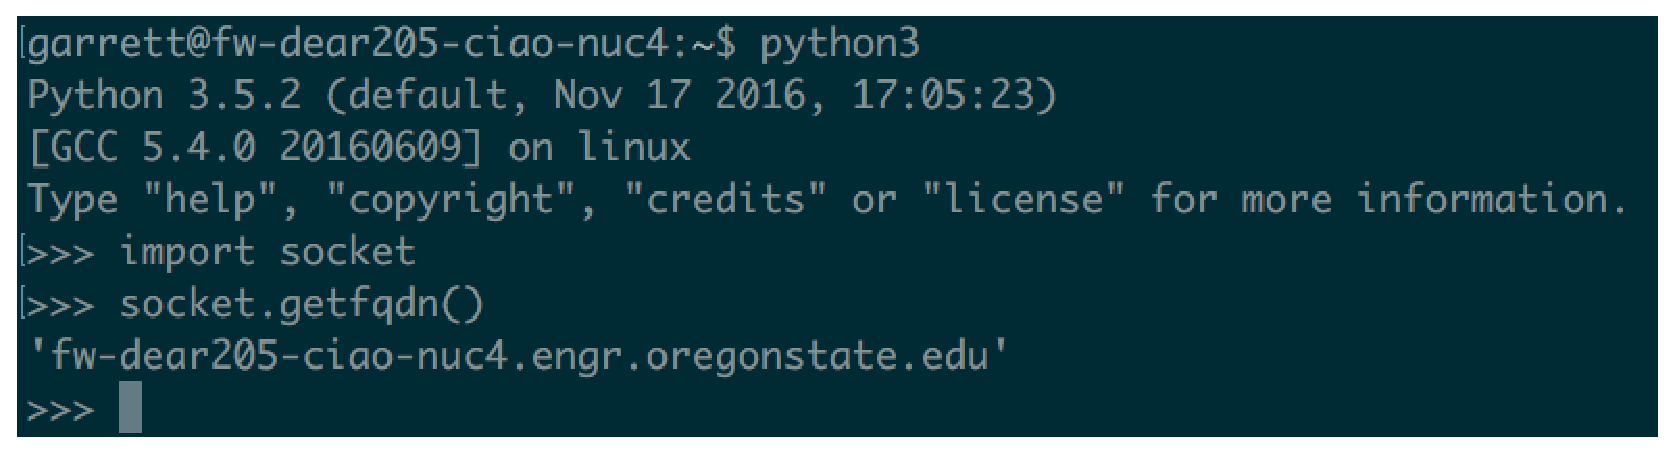
\includegraphics[scale=0.5]{getfqdn.eps}
\end{figure}

We found out later that the Ciao dev team usually uses Ubuntu as its development
environment. With that in mind, we decided to move to an Ubuntu development
environment to make it as consistent as possible. We have since then installed
Ubuntu 16.10 on all the machines. Also at the recommendation of the Ciao team,
we started using Ciao-Down, a single virtual machine development
environment. With this set up, we were able to quickly get to work on the 
development of the first feature. While we are not currently using a fully
deployed version of Ciao for development, we will work on getting Ciao tested
with the new features in our full five NUC setup once we've made progress on
development.

\subsection{Network Testing - Garrett Smith}

Using the automated deployment 
Ansible play book we were able to deploy Ciao, but we ran into errors running 
workloads using the Ciao command line interface. For example running 
\texttt{ciao-cli instance add -workload } resulted in the following error 
message.
\begin{lstlisting}[caption = Failing to run a workload]
garrett@fw-dear205-ciao-nuc1:~\$ ciao-cli instance add -workload ab68111c-03a6-11e6-87de-001320fb6e31 -instances 1
F0202 09:02:18.353666    8527 instance.go:531] ciao-cli FATAL: HTTP Error [500] for [POST https://fw-dear205-ciao-nuc1.engr.oregonstate.edu:8774/v2.1/8624fb4b8d8f489a9a32f051770aeed2/servers]: {"error":{"code":500,"name":"Internal Server Error","message":"Unable to Launch Tenant CNCI"}}
\end{lstlisting}

Garrett did some digging through the Ciao source code and located the source of 
the error as a new CNCI being created, but not receiving an IP address. We were 
running Ciao on the OSU network, which was not assigning an IP address to the 
CNCI.

To get more control over the network we are using Garrett set up an 
isolated local network using the Cisco SG300 switch Intel is lending us for the 
project, and is configuring Ciao on that. There are a few places
we had hostnames and other settings 
hardcoded into the deployment configuration. We need to update the 
configuration then we should be able to deploy Ciao onto the new network setup 
with the Ansible playbook.

\section{Winter Term Week by Week Reports - Matthew Johnson}
%just paste in weekly blogs?

\subsection{Winter Break and Week One}

Over Christmas break Cody and Matthew tried to get Ciao set up on the cluster
using a manual installation method. We ran into some tough issues and
communicated them with the Intel team. The Intel team pointed us to
a much more recently updated setup document that included automated deployment.

During week one there was still an issue in the version of Clear Linux (our
target distribution) that we were running that caused docker certification to be
broken. This was fixed within the week and we continued trying to set up Ciao.

\subsection{Week Two}

Garrett wrote several scripts to collect network performance data between nodes.
He made significant progress in parsing bandwidth data into csv format for
graphical representation.

This week we continued to work on the Ciao deployment via automated ansible
playbooks. We encountered several issues from the start and worked through
them one by one. Issues included errors in the ansible playbooks regarding yaml
parsing and fqdn configuration. This type of issue was resolved by hardcoding
the playbooks for our specific setup. By the end of the week we were seeing
certification management issues in the build.

\subsection{Week Three}

This week we believed we were successful in deploying Ciao and began implementation of
Open vSwitch components. Garrett has begun working out network measurements for
our initial benchmarks. Garrett discovered that the network was not being set up
properly, however, due to issues with the OSU network.

The first half of the week was spent debugging our Ciao deploy with members of
the Ciao development team at Intel. After several email conversations and debug
steps, we were advised to switch our operating system to Ubuntu because of
various certification issues in Clear Linux. This, along with running from
within a ciao-deploy docker container, fixed our issues and allowed us to
properly initialize the cluster. As mentioned earlier, our network was not
properly set up.

\subsection{Week Four}

During week four we continued tentative development on the OVS modules for Ciao.
Some of the necessary functions have been written, but it has been difficult to
test this over the physical cluster. Garrett, who has worked on the OSU network
in the past, thinks the network may not be assigning IPs to the cluster. The OSU
network DHCP servers will not assign an IP unless the MAC address has been
registered with the university. To get around this we may have to do single-vm
setup or find a way to set up the cluster independent from the OSU network.

Ciao provides ciao-down, a tool that helps set up a single-vm environment for
testing. This will be helpful once we get it spun up.

We were still having issues gathering initial network metrics due to inaccessible
nodes on our physical cluster. Garrett is working through this but the best way
to address this may be single-vm for now.

\subsection{Week Five}

Early in the week we got ciao-down (the single-vm setup for Ciao) working to
test our code.

We have a schedule we are following, and our initial goal was to complete the
OVS module by the end of week five. Although we had a module written of
something we were hoping might work, we were unable to get it to integrate
properly with the rest of Ciao.  It is likely we were misunderstanding some
things in the calling hierarchy.  Matthew communicated the issues we were seeing
with Manohar Castelino, one of our clients and a software defined networking
expert. This led to a conversation about whether or not it was strictly
necessary to create the bridges in Open vSwitch or if we could simply create the
GRE tunnels themselves.

As far as the physical cluster goes, we realized that the OSU network will not
lease IP addresses unless the MAC address is registered with the University.
Since Ciao uses the network's DHCP server to assign IP addresses to the nodes
this is a big issue. Garrett has been setting up the physical cluster with a
DHCP server running on the switch, with only our deployment NUC connected to the
internet. He has been running into issues setting up the Keystone server once he
took our controller NUC off the internet. He was trying to modify ansible tasks
to get around the issue when I left campus today. If he is not able to get this
to work we will probably ask the university for a subnet we can run a
non-MAC-locked DHCP server on, but Garrett has worked in OSU IT before and said
we are unlikely to get permission for that. The number of errors the OSU network
has generated for us has been a little frustrating.

\subsection{Week Six}

Matthew met with Manohar in-person at Intel on Tuesday to discuss the issues
with OVS bridges. It turns out Open vSwitch will not attach tunnels to non-OVS
bridges. This expands our scope somewhat to build a full OVS framework for Ciao,
instead of just OVS tunnels.

The rest of the week was devoted to working on the midterm progress report for
Winter term.

\section{Winter Midterm Retrospective}

\begin{center}
	\begin{tabular}{| p{0.05\linewidth} | p{0.3\linewidth} | p{0.3\linewidth} |
			p{0.3\linewidth} |}\hline
		Week & Positives & Deltas & Actions \\ \hline

		1 & Learned about automated deployment for Ciao & Worked through
		several deployment issues & Attempted to deploy Ciao \\ \hline

		2 & Scripts to collect network statistics completed & Resolved
		old issues in deployment but uncovered more & Hardcoding
		variables in the ansible deployment resolved some new issues \\
		\hline

		3 & Successfully initiated the cluster & Switched OS on the
		cluster to Ubunto & Started working in single-vm mode \\ \hline

		4 & Wrote some of the module for OVS tunnels & OSU network DHCP
		will not assign IPs to unregistered MACs & Developed in
		ciao-down \\ \hline

		5 & OVS module mostly written, but not integrated & Discussed
		whether OVS bridges were required for OVS tunnels & Tried to set
		up local DHCP server on switch \\ \hline

		6 & Met with Manohar regarding OVS bridges & OVS bridges are
		required for OVS tunnels & Worked on progress report for midterm
		\\ \hline

	\end{tabular}
\end{center}

\bibliographystyle{IEEEtran}
\bibliography{prog}

\end{document}
